\section{Use-case Model và Use-case Scenario}

Phần này gồm một sơ đồ use case toàn hệ thống và 18 bộ sơ đồ chi tiết -- đặc tả tương ứng với 18 use case trong danh mục. Mỗi phân hệ được mở đầu bằng phạm vi, actor và dependency chung; sau đó từng use case được trình bày bằng sơ đồ chi tiết và Use Case Specification.

\subsection{Mô hình use case toàn hệ thống}

\subsubsection{Actor Catalog}

\begin{table}[htbp]
  \centering
  \caption{Actor của Smart E-Mobility Hub}
  \label{tab:actors}
  \begin{tabularx}{\textwidth}{|L{22mm}|L{34mm}|Y|L{40mm}|}
    \hline
    \rowcolor{gray!15}
    \textbf{Mã} & \centering\arraybackslash\textbf{Actor} & \centering\arraybackslash\textbf{Mục tiêu chính} & \centering\arraybackslash\textbf{Phân hệ tương tác}\\
    \hline
    ACT-STU & Sinh viên & Tìm và sử dụng xe dùng chung; đặt chỗ đỗ, đăng ký sạc và theo dõi tài nguyên cho xe cá nhân. & HUB, RES, TRIP, PARK, CHG\\\hline
    ACT-OPR & Nhân viên vận hành & Giám sát mạng lưới Hub, quản lý sạc, xử lý sự cố, điều phối tài nguyên và chạy mô phỏng. & CHG, OPS, SIM\\\hline
    ACT-MNT & Nhân viên kỹ thuật & Tiếp nhận công việc kỹ thuật, cập nhật kết quả khắc phục và xác nhận tài nguyên đủ điều kiện trở lại phục vụ. & OPS\\\hline
    ACT-DAT & IoT \& State Data Gateway & Cung cấp trạng thái xe, mức pin, chỗ đỗ, cổng sạc và sự kiện vận hành từ \texttt{EXT-STATE}. & HUB, TRIP, PARK, CHG, OPS\\\hline
  \end{tabularx}
\end{table}

\clearpage
\subsubsection{Danh mục 18 use case}

\begin{longtable}{|L{26mm}|L{58mm}|L{25mm}|L{25mm}|}
  \caption{Danh mục use case toàn hệ thống}\label{tab:system-use-cases}\\
  \hline
  \rowcolor{gray!15}
  \textbf{Use Case ID} & \centering\arraybackslash\textbf{Tên use case} & \textbf{Phân hệ} & \textbf{Actor chính}\\
  \hline
  \endfirsthead
  \hline
  \rowcolor{gray!15}
  \textbf{Use Case ID} & \centering\arraybackslash\textbf{Tên use case} & \textbf{Phân hệ} & \textbf{Actor chính}\\
  \hline
  \endhead
  UC-HUB-01 & Tra cứu Hub phù hợp & SUB-HUB & ACT-STU\\\hline
  UC-HUB-02 & Xem trạng thái tài nguyên tại Hub & SUB-HUB & ACT-STU\\\hline
  UC-HUB-03 & Xem Hub thay thế & SUB-HUB & ACT-STU\\\hline
  UC-RES-01 & Đặt phương tiện dùng chung & SUB-RES & ACT-STU\\\hline
  UC-RES-02 & Hủy lượt đặt phương tiện & SUB-RES & ACT-STU\\\hline
  UC-TRIP-01 & Nhận phương tiện đã đặt & SUB-TRIP & ACT-STU\\\hline
  UC-TRIP-02 & Trả phương tiện và kết thúc chuyến đi & SUB-TRIP & ACT-STU\\\hline
  UC-PARK-01 & Đặt chỗ đỗ cho xe cá nhân & SUB-PARK & ACT-STU\\\hline
  UC-PARK-02 & Check-in phương tiện cá nhân & SUB-PARK & ACT-STU\\\hline
  UC-PARK-03 & Check-out phương tiện cá nhân & SUB-PARK & ACT-STU\\\hline
  UC-CHG-01 & Đăng ký nhu cầu sạc & SUB-CHG & ACT-STU, ACT-OPR\\\hline
  UC-CHG-02 & Theo dõi lịch và phiên sạc & SUB-CHG & ACT-STU, ACT-OPR\\\hline
  UC-CHG-03 & Điều chỉnh lịch sạc ưu tiên & SUB-CHG & ACT-OPR\\\hline
  UC-OPS-01 & Giám sát mạng lưới Mobility Hub & SUB-OPS & ACT-OPR\\\hline
  UC-OPS-02 & Xử lý sự cố vận hành & SUB-OPS & ACT-OPR\\\hline
  UC-OPS-03 & Điều phối phương tiện giữa các Hub & SUB-OPS & ACT-OPR\\\hline
  UC-SIM-01 & Chạy kịch bản What-if Simulation & SUB-SIM & ACT-OPR\\\hline
  UC-SIM-02 & Phân tích kết quả và khuyến nghị điều phối & SUB-SIM & ACT-OPR\\\hline
\end{longtable}

\clearpage
\subsubsection{Use-case Diagram toàn hệ thống}

Cấu trúc và quan hệ nghiệp vụ giữa bảy phân hệ đã được trình bày tại Hình~\ref{fig:subsystem-map}. Sơ đồ use case toàn hệ thống dưới đây khái quát các actor và bảy nhóm chức năng cấp cao tương ứng với bảy phân hệ. Danh mục 18 use case được trình bày tại Bảng~\ref{tab:system-use-cases} và được đặc tả chi tiết trong các mục tiếp theo.

\noindent\begin{minipage}{\linewidth}
  \centering
  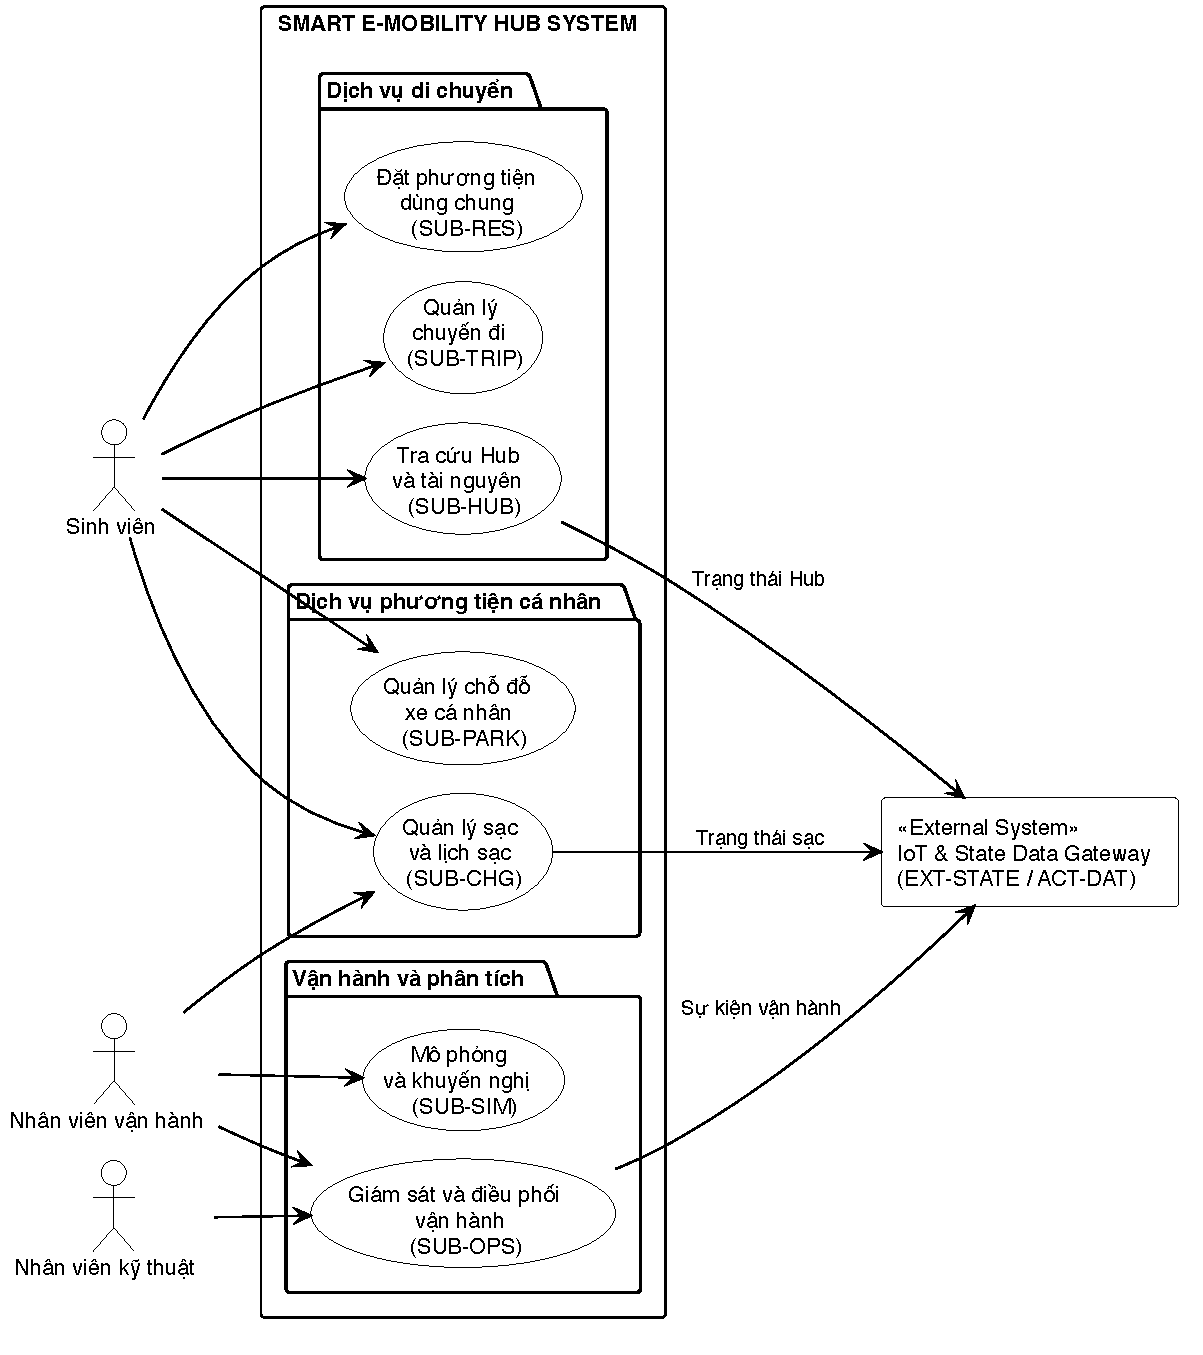
\includegraphics[height=0.73\textheight,keepaspectratio]{../diagrams/plantuml/output/system-use-case.pdf}
  \captionof{figure}{Use-case Diagram tổng quát của Smart E-Mobility Hub}
  \label{fig:system-use-case}
\end{minipage}\par\medskip

\newcommand{\SubsystemHeader}[5]{%
  \clearpage
  \subsection{SUB-#1 -- #2}
  \OwnerNote{#3 -- #4}
  \noindent\textbf{Các use case được giao:} #5

  \paragraph{Phạm vi, actor và dependency.}
  \Placeholder{Mô tả trách nhiệm của phân hệ, actor tham gia, dữ liệu đầu vào, kết quả đầu ra và dependency với phân hệ khác.}
}

\newcommand{\UseCaseSpecification}[5]{%
  \subsubsection{#1 -- #2}
  \OwnerNote{#5}

  \UseCaseDiagramPlaceholder{#1}{#2}{fig:uc-#1}

  \paragraph{Đặc tả Use Case (Use Case Specification).}
  \small
  \begin{longtable}{|L{42mm}|L{102mm}|}
    \caption{Đặc tả Use Case #1 -- #2}\label{tab:spec-#1}\\
    \hline
    \rowcolor{gray!15}
    \centering\arraybackslash\textbf{Trường} & \centering\arraybackslash\textbf{Nội dung}\\
    \hline
    \endfirsthead
    \hline
    \rowcolor{gray!15}
    \centering\arraybackslash\textbf{Trường} & \centering\arraybackslash\textbf{Nội dung (tiếp theo)}\\
    \hline
    \endhead
    Use Case ID & #1\\\hline
    Use Case Name & #2\\\hline
    Owning Subsystem & #3\\\hline
    Actors & \textbf{Primary:} #4. \textbf{Supporting:} \Placeholder{ACT/EXT liên quan hoặc Không có}.\\\hline
    Description / Goal & \Placeholder{Mô tả ngắn mục tiêu nghiệp vụ và giá trị actor nhận được khi use case hoàn tất.}\\\hline
    Trigger & \Placeholder{Sự kiện bắt đầu use case.}\\\hline
    Preconditions & \Placeholder{Liệt kê các điều kiện phải đúng trước khi bắt đầu.}\\\hline
    Postconditions & \textbf{Thành công:} \Placeholder{Trạng thái sau khi hoàn tất}. \newline
      \textbf{Thất bại:} \Placeholder{Trạng thái được bảo toàn hoặc khôi phục}.\\\hline
    Main Flow &
      \textbf{1.} \Placeholder{Actor gửi yêu cầu hoặc bắt đầu tác vụ.}\newline
      \textbf{2.} \Placeholder{Hệ thống kiểm tra dữ liệu và điều kiện nghiệp vụ.}\newline
      \textbf{3.} \Placeholder{Actor xác nhận hoặc cung cấp thông tin tiếp theo.}\newline
      \textbf{4.} \Placeholder{Hệ thống xử lý và trả kết quả cuối cùng.}\newline
      \Placeholder{Thêm bước nếu cần; mỗi bước phải thể hiện rõ bên thực hiện.}\\\hline
    Alternative Flows & \textbf{AF-01 -- \Placeholder{Tên luồng thay thế}.} \textit{Rẽ từ bước \Placeholder{N}.} \Placeholder{Mô tả điều kiện, diễn biến và điểm quay lại hoặc kết quả.}\\\hline
    Exception Flows & \textbf{EF-01 -- \Placeholder{Tên ngoại lệ}.} \textit{Phát sinh tại bước \Placeholder{N}.} \Placeholder{Mô tả lỗi, phản hồi và trạng thái dữ liệu sau lỗi.}\\\hline
    Related Requirements & \Placeholder{FR cùng phân hệ và NFR có liên quan.}\\\hline
    Related Business Rules & \Placeholder{BR cùng phân hệ.}\\\hline
    Dependencies & \Placeholder{SUB/UC liên quan hoặc Không có.}\\\hline
  \end{longtable}
  \normalsize
  \clearpage
}

\SubsystemHeader{HUB}{Tra cứu Hub và tài nguyên}{Nguyễn Quốc Trung}{2413707}{UC-HUB-01, UC-HUB-02 và UC-HUB-03}
\UseCaseSpecification{UC-HUB-01}{Tra cứu Hub phù hợp}{SUB-HUB}{ACT-STU}{Nguyễn Quốc Trung -- 2413707}
\UseCaseSpecification{UC-HUB-02}{Xem trạng thái tài nguyên tại Hub}{SUB-HUB}{ACT-STU}{Nguyễn Quốc Trung -- 2413707}
\UseCaseSpecification{UC-HUB-03}{Xem Hub thay thế}{SUB-HUB}{ACT-STU}{Nguyễn Quốc Trung -- 2413707}

\SubsystemHeader{RES}{Đặt phương tiện dùng chung}{Phan Võ Bảo Trâm}{2413576}{UC-RES-01 và UC-RES-02}
\UseCaseSpecification{UC-RES-01}{Đặt phương tiện dùng chung}{SUB-RES}{ACT-STU}{Phan Võ Bảo Trâm -- 2413576}
\UseCaseSpecification{UC-RES-02}{Hủy lượt đặt phương tiện}{SUB-RES}{ACT-STU}{Phan Võ Bảo Trâm -- 2413576}

\SubsystemHeader{TRIP}{Quản lý chuyến đi}{Lê Nguyễn Tường Vi}{2413937}{UC-TRIP-01 và UC-TRIP-02}
\UseCaseSpecification{UC-TRIP-01}{Nhận phương tiện đã đặt}{SUB-TRIP}{ACT-STU}{Lê Nguyễn Tường Vi -- 2413937}
\UseCaseSpecification{UC-TRIP-02}{Trả phương tiện và kết thúc chuyến đi}{SUB-TRIP}{ACT-STU}{Lê Nguyễn Tường Vi -- 2413937}

\SubsystemHeader{PARK}{Quản lý chỗ đỗ xe cá nhân}{Nguyễn Ngọc Hân}{2410951}{UC-PARK-01, UC-PARK-02 và UC-PARK-03}
\UseCaseSpecification{UC-PARK-01}{Đặt chỗ đỗ cho xe cá nhân}{SUB-PARK}{ACT-STU}{Nguyễn Ngọc Hân -- 2410951}
\UseCaseSpecification{UC-PARK-02}{Check-in phương tiện cá nhân}{SUB-PARK}{ACT-STU}{Nguyễn Ngọc Hân -- 2410951}
\UseCaseSpecification{UC-PARK-03}{Check-out phương tiện cá nhân}{SUB-PARK}{ACT-STU}{Nguyễn Ngọc Hân -- 2410951}

\SubsystemHeader{CHG}{Quản lý sạc và lịch sạc}{Trần Thị Hương Giang}{2410845}{UC-CHG-01, UC-CHG-02 và UC-CHG-03}
\UseCaseSpecification{UC-CHG-01}{Đăng ký nhu cầu sạc}{SUB-CHG}{ACT-STU, ACT-OPR}{Trần Thị Hương Giang -- 2410845}
\UseCaseSpecification{UC-CHG-02}{Theo dõi lịch và phiên sạc}{SUB-CHG}{ACT-STU, ACT-OPR}{Trần Thị Hương Giang -- 2410845}
\UseCaseSpecification{UC-CHG-03}{Điều chỉnh lịch sạc ưu tiên}{SUB-CHG}{ACT-OPR}{Trần Thị Hương Giang -- 2410845}

\SubsystemHeader{OPS}{Giám sát và điều phối vận hành}{Nguyễn Thị Minh Anh}{2410126}{UC-OPS-01, UC-OPS-02 và UC-OPS-03}
\UseCaseSpecification{UC-OPS-01}{Giám sát mạng lưới Mobility Hub}{SUB-OPS}{ACT-OPR}{Nguyễn Thị Minh Anh -- 2410126}
\UseCaseSpecification{UC-OPS-02}{Xử lý sự cố vận hành}{SUB-OPS}{ACT-OPR}{Nguyễn Thị Minh Anh -- 2410126}
\UseCaseSpecification{UC-OPS-03}{Điều phối phương tiện giữa các Hub}{SUB-OPS}{ACT-OPR}{Nguyễn Thị Minh Anh -- 2410126}

\SubsystemHeader{SIM}{What-if Simulation và khuyến nghị}{Trần Nhật Bảo Anh}{2410155}{UC-SIM-01 và UC-SIM-02}
\UseCaseSpecification{UC-SIM-01}{Chạy kịch bản What-if Simulation}{SUB-SIM}{ACT-OPR}{Trần Nhật Bảo Anh -- 2410155}
\UseCaseSpecification{UC-SIM-02}{Phân tích kết quả và khuyến nghị điều phối}{SUB-SIM}{ACT-OPR}{Trần Nhật Bảo Anh -- 2410155}

\clearpage
